\section{Model}

\subsection{Text Classification}

We propose a deep neural model to capture linguistics partern of the text. This model is based on simple Convolutional Neural Network with an embedding layer for words representaion, one covolutional with pooling layer and finnaly one Dense layer. Figure \ref{cnn} shows the global structure of our architecture. The input is a sequence of words $ w_{1}, w_{2} ... w_{n} $ and the output contains class element (for text classification). The embedding is build on top of a Word2Vec architecture trained on a Skip-gram model. Our text tokenizer keeps all the words to make sure all linguistics material could be detected at the end by the model. This embedding is also trainable by the model to reach the best text-classification acuracy. 

The Convolutional layer is based on a 2 dimensionals convolution, the same as used for pictures convolution, but with a fixed width corresponding to the max width (this size is actually equal to the embedding size). With this setting, our usage of the 2 dimensionals convolution is in reallity the same as a 1 dimensional convolution (the default convolutionnal layer for text). The only parameter we adjuste here is the height of the filter corresponding to the number of words we want to put in the filter. The goal of this approach is to be able to use the standard picture deconvolution (conv2D Transpose) methods for our model on text.

The last layer is a fully connected dense network (with one hidden layer) finishing on a output size corresponding to the number of class we attempt to train.

\subsection{Deconvolution}

Since we use same architecture as image detection, making a deconvolutional layer is really straightforward. There are several methods to visualize the deep internal mecanisms of a neural network. One is called convolutional transposed. Our deconvolutional network use the same embedding and convolution layer as we use for the classification but we replace the finale dense layer by a convolutional transposed layer (also called deconvolution). After we trained the model we setup the weight of each neuron of the deconvolutional network with the learned weights of the classification network. The result is a new network that takes in input a sequence of words and gives us in output all the trained filters of the text classification applied on the given sequence. Then the activation score of each word is calculated as shown in Equation \ref{equation} with $x$ is the size of the embedding, and $y$ the number of applied filters : 

\begin{equation}
\mathop{\sum^{x}\sum^{y}}_{i=1  j=1}  a_{ij} = s_{n}
\label{equation}
\end{equation}

\begin{figure}[h]
\begin{center}
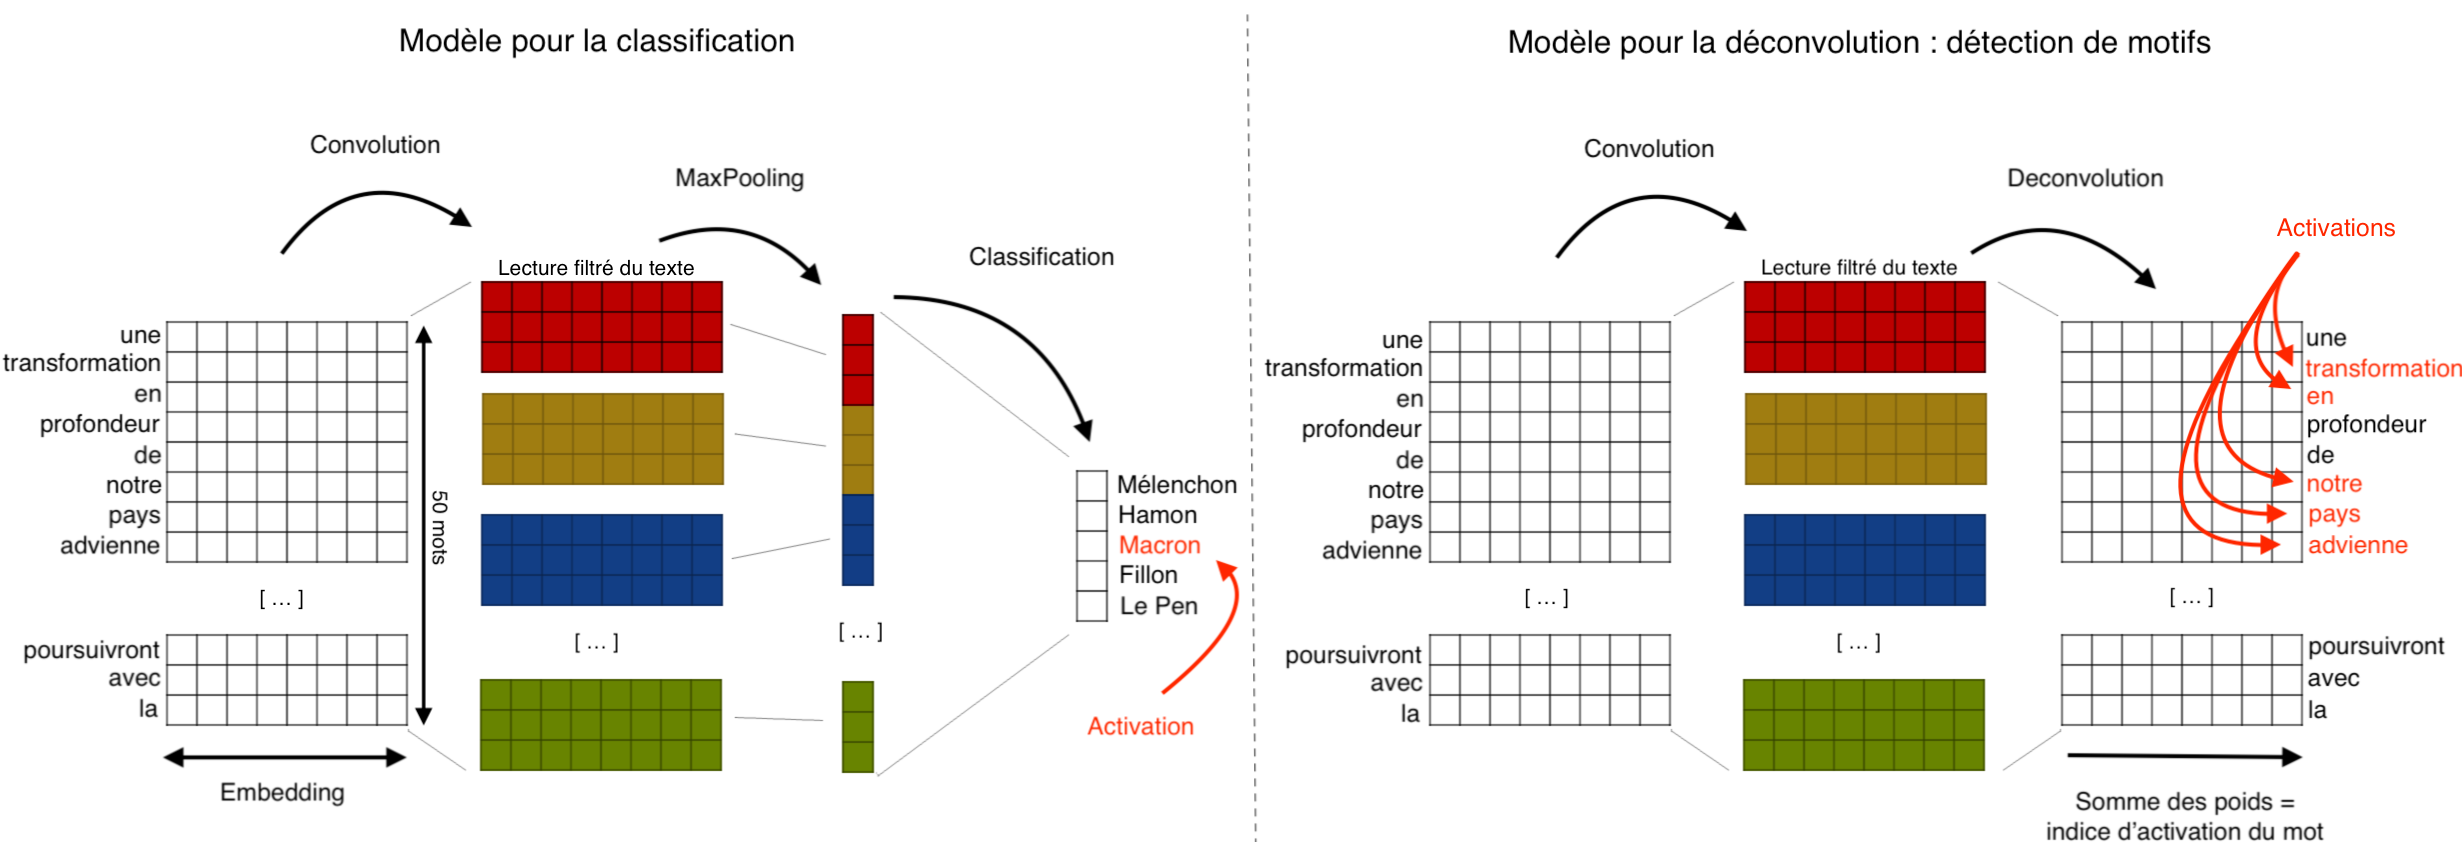
\includegraphics[width=16cm]{img/model.png}
\caption{Deconvolution model}
\label{cnn}
\end{center}
\end{figure}

With this method we are able to show a sort of topology of a sequence of words. All words have an unique activation score related to the others. We going to see now that this output of the deconvolution give us many information on how the network takes his final descision (prediction). There're well known linguistics marks encoded inside but also some more complexe pattern based on cooccurrences and maybe also on grammatical and syntaxic analysis.
